\documentclass[12pt]{article}

\usepackage[utf8]{inputenc}
\usepackage[T1]{fontenc}
\usepackage[a4paper, margin=1in]{geometry}  
\usepackage{graphicx}
\usepackage{hyperref}
\usepackage{float} % For [H] option in figures

\title{Anotacja korpusów oraz osadzenia słów i tekstów\\Część II: Modele przestrzeni wektorowych}
\author{Autorzy: Oliwer Krupa, Adam Bednarski, Jan Masłowski, Łukasz Lenkiewicz}
\date{\today}

\begin{document}

\maketitle
\newpage

\tableofcontents
\newpage

\section{Word Embeddings}

\subsection{Osadzenia słów w anotowanym korpusie (Word2Vec i Fasttext)}

W celu zbadania i wizualizacji osadzeń słów w anotowanym korpusie, zastosowaliśmy dwie metody: \textbf{Word2Vec} oraz \textbf{FastText}. Dla obu modeli osadziliśmy słowa, a następnie zwizualizowaliśmy wyniki za pomocą algorytmu t-SNE, który redukuje wymiary danych, co pozwala na łatwiejszą analizę i porównanie rezultatów.

\subsubsection{Word2Vec}
Model \textbf{Word2Vec} został przetrenowany na korpusie tekstów polskich, a następnie osadziliśmy słowa z anotowanego korpusu, aby sprawdzić, jak różne słowa są reprezentowane w przestrzeni wektorowej. Wyniki zostały przedstawione na poniższym wykresie, gdzie kolory reprezentują różne kategorie sentymentu — niektóre słowa zostały oznaczone jako "Brak etykiety", a inne jako "Wzmacnianie".

\begin{figure}[H]
    \centering
    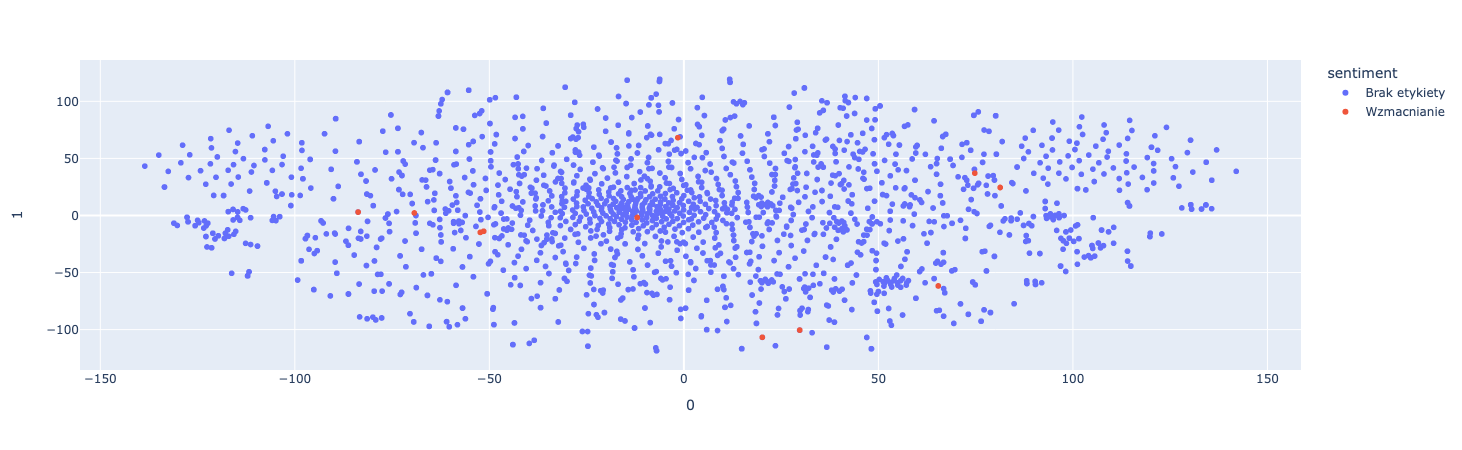
\includegraphics[width=\textwidth]{../../plots/w2v-word.png}
    \caption{Wizualizacja osadzeń słów za pomocą Word2Vec}
    \label{fig:w2v_word}
\end{figure}

Jak widać na rysunku \ref{fig:w2v_word}, większość słów jest zgrupowana w centralnej części wykresu, jednak niektóre słowa przypisane do kategorii "Wzmacnianie" znajdują się różnych obrszarach przestrzeni wektorowej.

\subsubsection{FastText}
Podobną analizę przeprowadzono z użyciem modelu \textbf{FastText}, który również został przetrenowany na korpusie polskim. Wyniki osadzeń słów z tego modelu zostały przedstawione na poniższym wykresie, który podobnie jak poprzedni, został wygenerowany za pomocą t-SNE.

\begin{figure}[H]
    \centering
    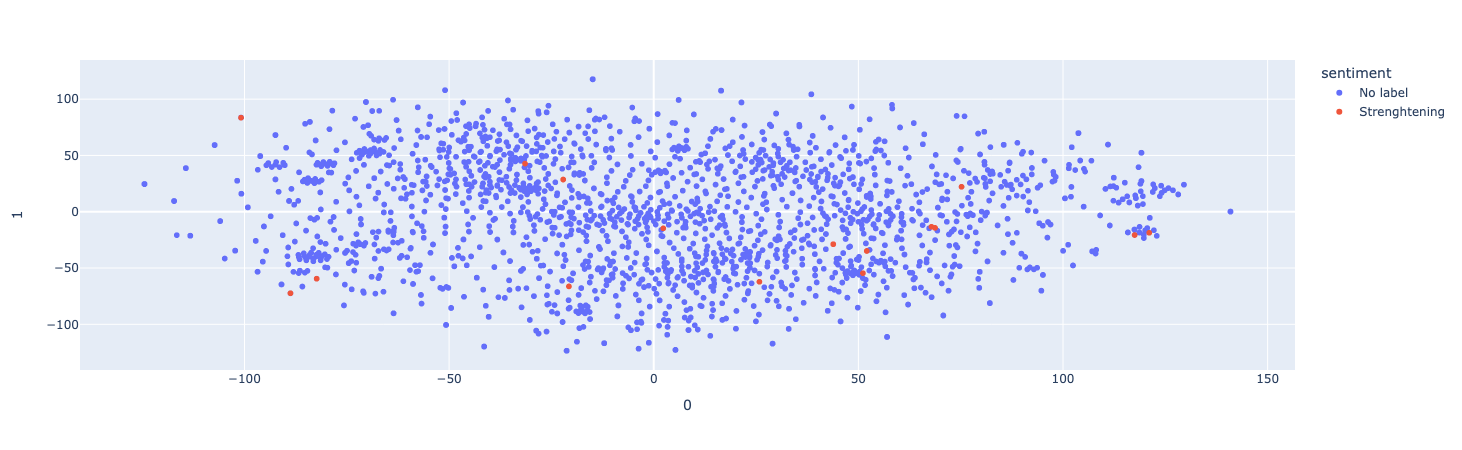
\includegraphics[width=\textwidth]{../../plots/ft-word.png}
    \caption{Wizualizacja osadzeń słów za pomocą FastText}
    \label{fig:ft_word}
\end{figure}

Rysunek \ref{fig:ft_word} pokazuje, że wyniki dla modelu FastText są podobne do tych uzyskanych z Word2Vec, chociaż niektóre grupy słów znajdują się w różnych częściach przestrzeni, co wynika z różnic w sposobie reprezentacji słów przez te dwa modele.

\subsection{Porównanie k-najbardziej podobnych słów dla modeli Word2Vec i FastText}

W ramach analizy wygenerowano listy pięciu najbardziej podobnych słów dla zaanotowanych terminów, wykorzystując modele \textbf{Word2Vec} oraz \textbf{FastText}. Wyniki pokazują różnice w sposobie modelowania podobieństw między słowami.

\subsubsection{Wyniki dla Word2Vec}
Dla modelu \textbf{Word2Vec}, lista najbardziej podobnych słów zawierała m.in.:
\begin{itemize}
    \item \textbf{by}: aby (0.89), żeby (0.86), więc (0.69)
    \item \textbf{kto}: dlaczego (0.66), czemu (0.63), jeśli (0.59)
    \item \textbf{człowiek}: osobnik (0.64), osoba (0.64), tubylec (0.62)
    \item \textbf{seks}: sexu (0.76), masturbacja (0.71), erotyka (0.63)
    \item \textbf{fakt}: stwierdzenie (0.66), twierdzenie (0.65), hipoteza (0.59)
\end{itemize}

\subsubsection{Wyniki dla FastText}
Dla modelu \textbf{FastText}, podobne słowa to:
\begin{itemize}
    \item \textbf{by}: By (0.77), żeby (0.61), muc (0.60)
    \item \textbf{kto}: Kto (0.80), ktoś (0.78), ktokolwiek (0.72)
    \item \textbf{człowiek}: Człowiek (0.80), czlowiek (0.76), człowiek. (0.69)
    \item \textbf{seks}: sex (0.80), seks. (0.78), seks- (0.76)
    \item \textbf{fakt}: faktem (0.68), faktu (0.66), Fakt (0.65)
\end{itemize}

\subsubsection{Dyskusja wyników}
Oba modele pokazują różnice w sposobie reprezentacji podobieństw. \textbf{FastText} lepiej radzi sobie z różnymi formami morfologicznymi i fleksyjnymi, np. dla słowa „człowiek” uwzględnia różne jego odmiany. Z kolei \textbf{Word2Vec} ma tendencję do generowania bardziej ogólnych podobieństw, co sprawia, że jest mniej precyzyjny w przypadku rzadkich wyrażeń. FastText dzięki n-gramom lepiej odwzorowuje złożoność morfologiczną języka polskiego.

\section{Text Embeddings}

\section{Osadzenia zdań za pomocą dwóch różnych modeli i wizualizacja t-SNE}

W ramach tej części eksperymentu wygenerowano osadzenia zdań z anotowanego korpusu, wykorzystując dwa różne modele: \textbf{TF-IDF} oraz \textbf{BERT}. Następnie wyniki osadzeń zostały zwizualizowane za pomocą algorytmu \textbf{t-SNE}, który redukuje wymiary danych, ułatwiając analizę i porównanie osadzeń zdań.

\subsection{TF-IDF}

Model \textbf{TF-IDF} (ang. Term Frequency-Inverse Document Frequency) mierzy częstość występowania słowa w danym dokumencie w stosunku do jego częstości w całym korpusie. Jest to popularny model bazujący na statystycznym podejściu, który nadaje większe wagi słowom występującym rzadziej w całym korpusie, co pozwala na lepsze odwzorowanie kluczowych informacji w osadzeniach tekstów.

Wizualizacja uzyskanych osadzeń za pomocą algorytmu t-SNE dla modelu TF-IDF jest przedstawiona na Rysunku \ref{fig:tfidf_tsne}. Kolory punktów odpowiadają różnym kategoriom sentymentu: "Mowa nienawiści" (kolor czerwony) oraz "Neutralny" (kolor niebieski). Każdy punkt na wykresie reprezentuje jedno zdanie z korpusu, a po najechaniu na punkt można odczytać treść zdania. Poza tesśćią można zauważyć 'sentiment' czyli etykietę sentymentu przypisaną do danego zdania.

\begin{figure}[H]
    \centering
    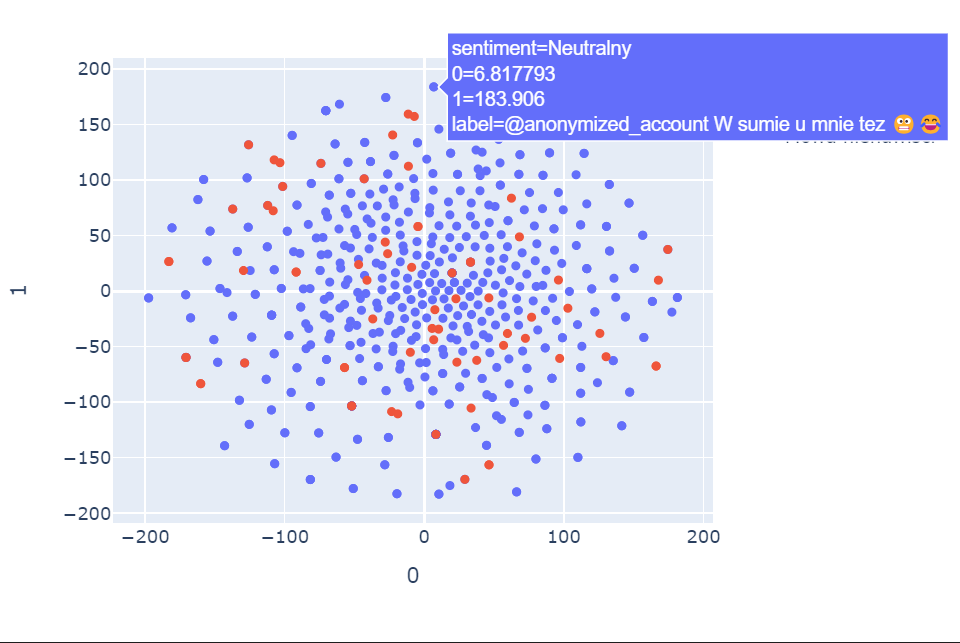
\includegraphics[width=\textwidth]{../../plots/tf-idf-t-sne.png}
    \caption{Wizualizacja osadzeń zdań za pomocą modelu TF-IDF przy użyciu t-SNE}
    \label{fig:tfidf_tsne}
\end{figure}

\subsection{BERT}

Model \textbf{BERT} (ang. Bidirectional Encoder Representations from Transformers) jest jednym z najnowocześniejszych modeli do przetwarzania języka naturalnego, wykorzystującym głębokie sieci neuronowe typu transformer. BERT jest w stanie generować osadzenia zdań z uwzględnieniem kontekstu zarówno przed, jak i po danym słowie, co czyni go bardziej skutecznym w modelowaniu złożonych relacji semantycznych w tekście.

Rysunek \ref{fig:bert_tsne} przedstawia wyniki osadzeń zdań wygenerowanych przy użyciu modelu BERT, zwizualizowane za pomocą t-SNE. Podobnie jak w przypadku TF-IDF, kolory odpowiadają różnym kategoriom sentymentu, a każdy punkt reprezentuje jedno zdanie.

\begin{figure}[H]
    \centering
    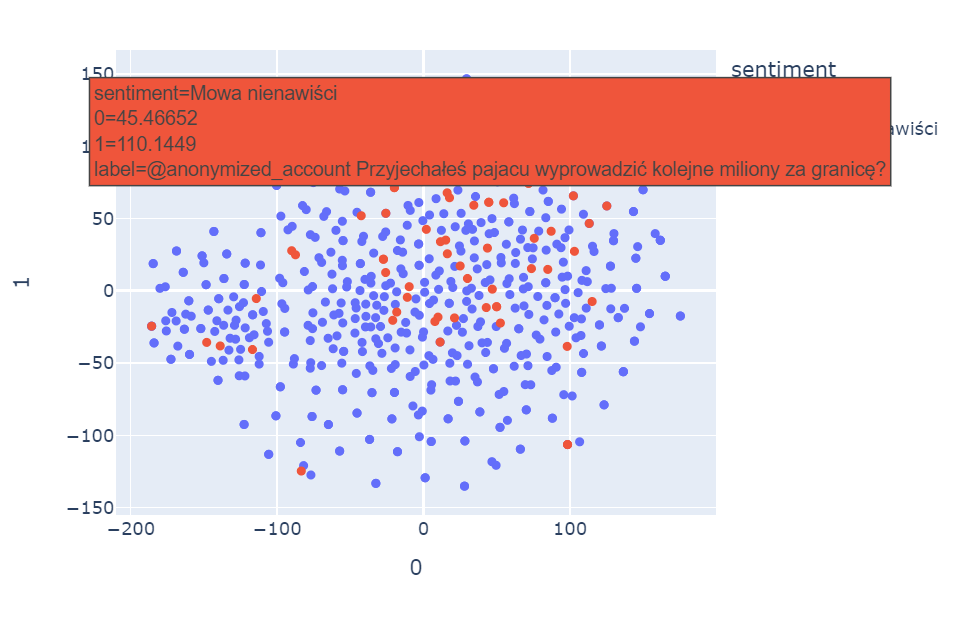
\includegraphics[width=\textwidth]{../../plots/bert-t-sne.png}
    \caption{Wizualizacja osadzeń zdań za pomocą modelu BERT przy użyciu t-SNE}
    \label{fig:bert_tsne}
\end{figure}

\subsection{Porównanie modeli}

Wyniki wizualizacji t-SNE dla modeli \textbf{TF-IDF} oraz \textbf{BERT} pokazują różne podejścia do modelowania osadzeń zdań. TF-IDF, bazując na częstościach słów, generuje osadzenia w sposób bardziej statystyczny, natomiast BERT, dzięki swoim zaawansowanym mechanizmom modelowania kontekstu, pozwala na lepsze uchwycenie semantycznych relacji między zdaniami. W obu przypadkach obserwujemy, że zdania oznaczone jako "Mowa nienawiści" są grupowane w określonych regionach przestrzeni, co może sugerować charakterystyczne cechy językowe używane w takich wypowiedziach.

\subsection{Klasteryzacja osadzeń anotowanych zdań}

W tej części zadania przeprowadziliśmy klasteryzację osadzeń anotowanych zdań uzyskanych z dwóch różnych modeli: TF-IDF oraz BERT. Do klasteryzacji zastosowano dwa różne algorytmy: \textbf{KMeans} oraz \textbf{HDBSCAN}. Wyniki klasteryzacji zostały przedstawione na wykresach t-SNE, które redukują wymiary wektorów osadzeń, umożliwiając wizualizację wyników w przestrzeni dwuwymiarowej.

\subsubsection{Klasteryzacja za pomocą KMeans}

Na pierwszym wykresie (Rysunek \ref{fig:kmeans_tf-idf}) przedstawiono wyniki klasteryzacji przy użyciu algorytmu KMeans dla osadzeń uzyskanych z modelu TF-IDF. Widać wyraźne grupowanie punktów odpowiadających różnym klastrom.

\begin{figure}[H]
    \centering
    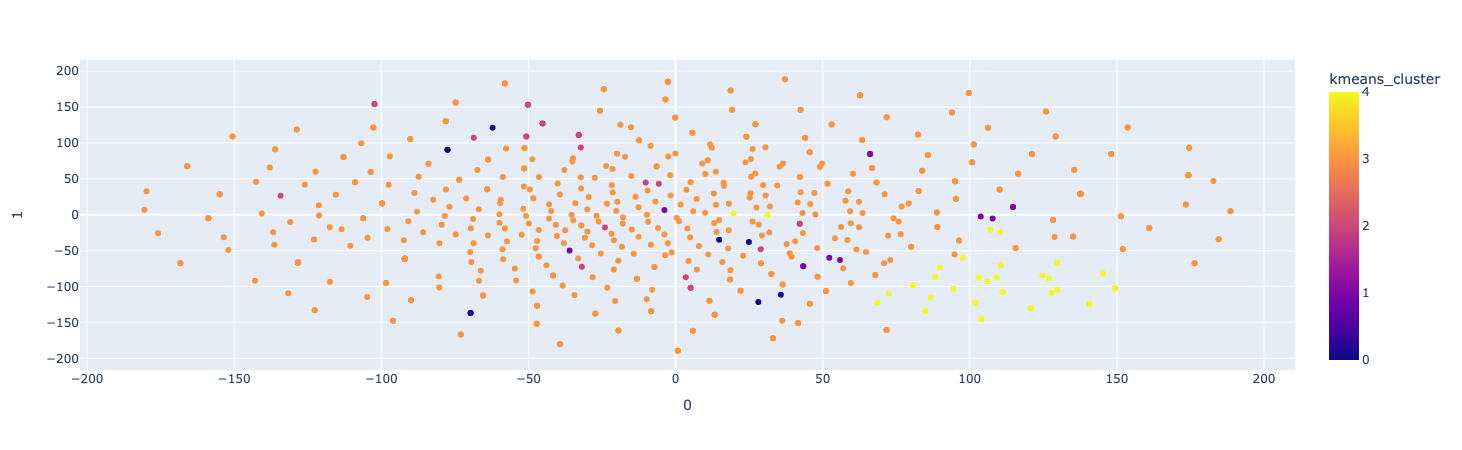
\includegraphics[width=\textwidth]{../../plots/tf-idf-kmeans-sentence.png}
    \caption{Klasteryzacja TF-IDF z użyciem algorytmu KMeans}
    \label{fig:kmeans_tf-idf}
\end{figure}

Podobną analizę przeprowadzono dla modelu BERT (Rysunek \ref{fig:kmeans_bert}), gdzie również widzimy wyraźne grupowanie zdań.

\begin{figure}[H]
    \centering
    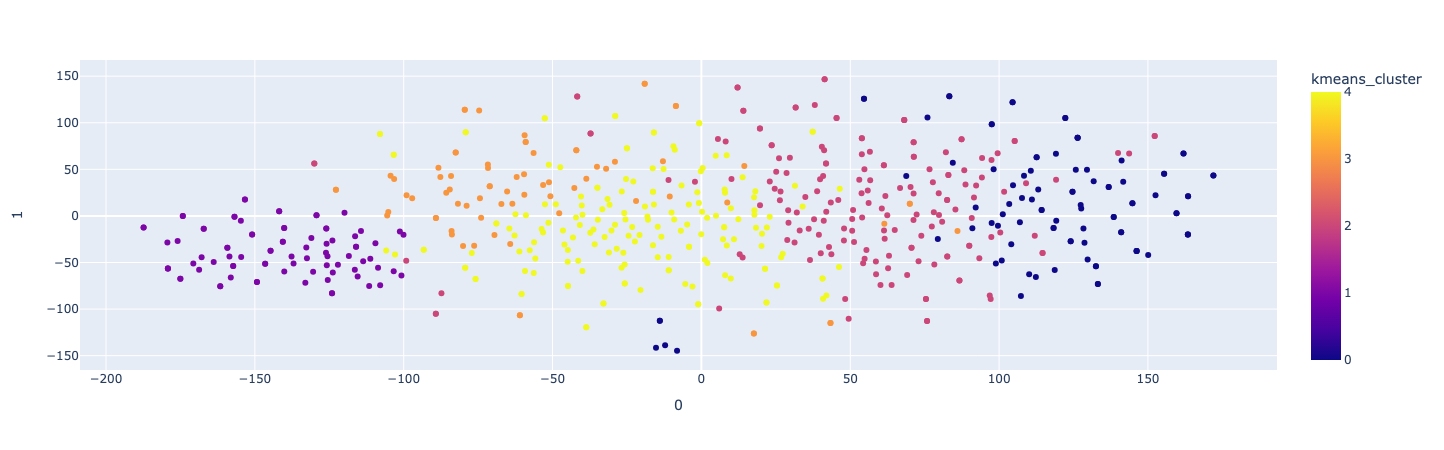
\includegraphics[width=\textwidth]{../../plots/bert-kmeans-sentence.png}
    \caption{Klasteryzacja BERT z użyciem algorytmu KMeans}
    \label{fig:kmeans_bert}
\end{figure}

\subsubsection{Klasteryzacja za pomocą HDBSCAN}

Dla porównania zastosowano również algorytm HDBSCAN, który jest nienadzorowanym algorytmem klasteryzacji potrafiącym identyfikować klastery o nieregularnych kształtach. Wyniki klasteryzacji modelu TF-IDF za pomocą HDBSCAN przedstawiono na Rysunku \ref{fig:hdbscan_tf-idf}, a dla BERT na Rysunku \ref{fig:hdbscan_bert}.

\begin{figure}[H]
    \centering
    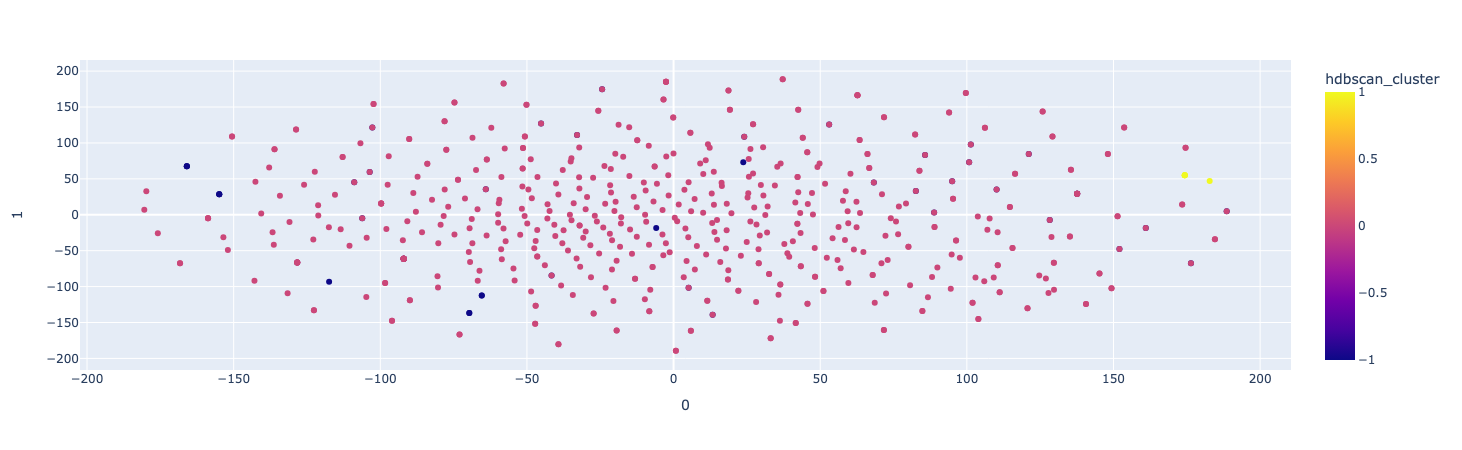
\includegraphics[width=\textwidth]{../../plots/tf-idf-hdbscan-sentence.png}
    \caption{Klasteryzacja TF-IDF z użyciem algorytmu HDBSCAN}
    \label{fig:hdbscan_tf-idf}
\end{figure}

\begin{figure}[H]
    \centering
    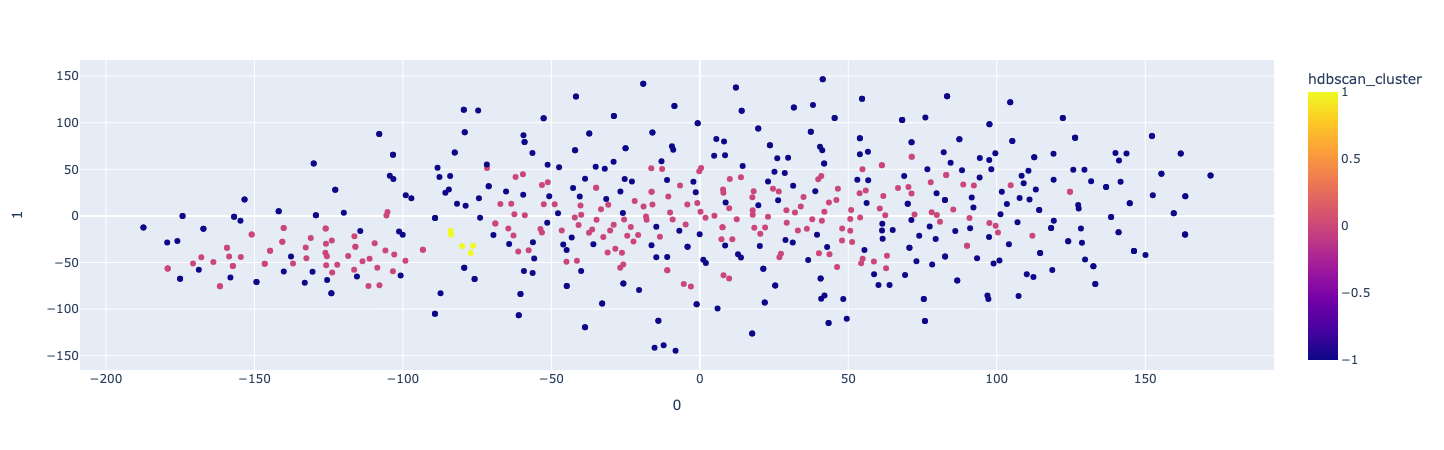
\includegraphics[width=\textwidth]{../../plots/bert-hdbscan-sentence.png}
    \caption{Klasteryzacja BERT z użyciem algorytmu HDBSCAN}
    \label{fig:hdbscan_bert}
\end{figure}

\subsubsection{Dyskusja wyników klasteryzacji}

Analizując wyniki klasteryzacji dla obu algorytmów, możemy zauważyć różnice w rozkładzie punktów na wykresach. KMeans wyraźnie dzieli przestrzeń na równe klastry, podczas gdy HDBSCAN jest bardziej elastyczny i potrafi identyfikować mniej regularne struktury klastrów.

\end{document}
